\documentclass[aspectratio=169,10pt]{beamer}
\usetheme{default}
\usecolortheme{default}
\setbeamertemplate{navigation symbols}{}
\setbeamertemplate{footline}{\hfill\insertframenumber{} / \inserttotalframenumber\hspace{1em}\vspace{0.8em}}
\setbeamertemplate{itemize items}[circle]
\usepackage[T1]{fontenc}
\usepackage{lmodern}
\usepackage{booktabs}
\usepackage{graphicx}
\usepackage{xcolor}
\graphicspath{{./}{topic2/}}

\definecolor{ink}{RGB}{30,45,58}
\definecolor{blueaccent}{RGB}{20,101,150}
\definecolor{greenaccent}{RGB}{54,122,68}
\setbeamercolor{structure}{fg=blueaccent}
\setbeamercolor{frametitle}{fg=ink}
\setbeamercolor{title}{fg=ink}
\setbeamercolor{normal text}{fg=ink}

\title{Deadlock-Free Adaptive Routing\\and Bubble Flow Control for a 3D Torus}
\subtitle{gem5 Garnet Lab 4 Project}
\author{Changxun Pan \and Liming Wang}
\institute{Computer Architecture}
\date{August 2026}

\begin{document}

\begin{frame}
  \titlepage
  \vspace{-0.3cm}
  \centering
\includegraphics[height=0.25in]{member_names.pdf}
\end{frame}

\begin{frame}{Problem and Scope}
  \begin{itemize}
    \item A 3D Torus shortens paths with wrap links, but those links create cyclic channel dependencies.
    \item Topic 1: add 3D Mesh/Torus topologies and a deadlock-free minimal adaptive Torus router.
    \item Topic 2: add Critical Bubble Scheme (CBS) flow control to protect deterministic Torus DOR without reserving a VC.
  \end{itemize}
  \vspace{0.4cm}
  \begin{block}{Central idea}
    Keep a connected, acyclic progress path at the routing layer, or preserve one movable free slot at the flow-control layer.
  \end{block}
\end{frame}

\begin{frame}{3D Torus Implementation}
  \begin{columns}[T]
    \begin{column}{0.48\textwidth}
      \begin{itemize}
        \item Parameterized \texttt{Mesh3D.py} and \texttt{Torus3D.py}.
        \item Evaluation instance: $4\times4\times4=64$ routers.
        \item Router ID: $zXY+yX+x$.
        \item 3D Mesh: 144 undirected neighbour pairs.
        \item 3D Torus: 192 pairs, adding 33.3\% wrap connectivity.
      \end{itemize}
    \end{column}
    \begin{column}{0.48\textwidth}
      \begin{tabular}{cl}
        \toprule
        ID & Policy \\
        \midrule
        3 & Torus minimal XYZ DOR \\
        4 & Torus adaptive + Escape VC \\
        5 & Mesh non-wrap XYZ \\
        \bottomrule
      \end{tabular}
      \vspace{0.5cm}
      \begin{block}{Controlled comparison}
        Torus DOR versus Torus adaptive keeps the topology, clocks, packet type, and total VC count fixed.
      \end{block}
    \end{column}
  \end{columns}
\end{frame}

\begin{frame}{Topic 1: Adaptive Routing with Escape VCs}
  \begin{columns}[T]
    \begin{column}{0.64\textwidth}
      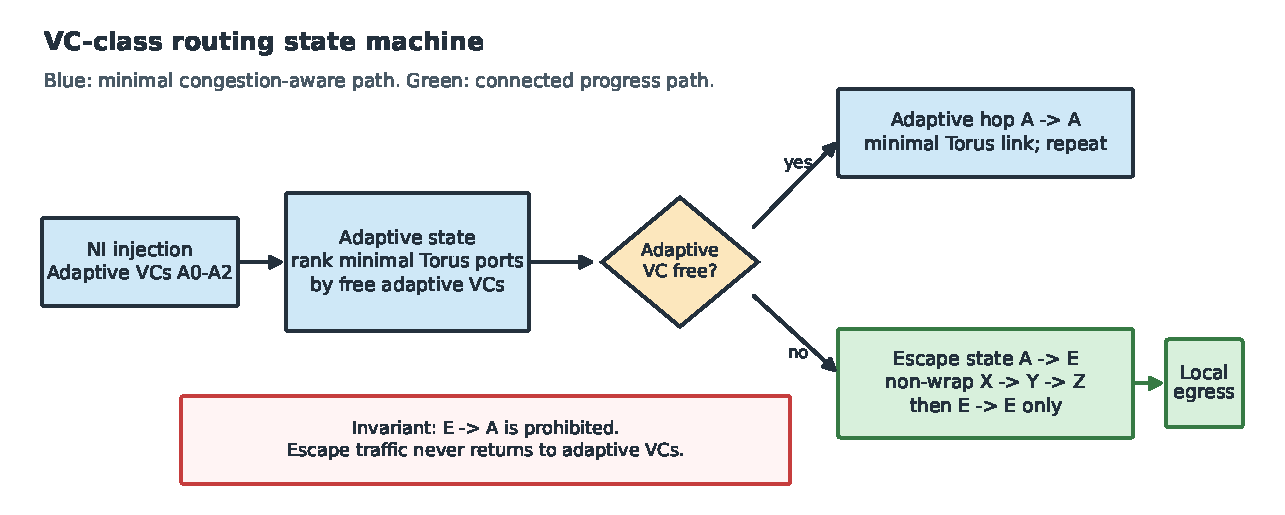
\includegraphics[width=\linewidth]{routing_architecture.pdf}
    \end{column}
    \begin{column}{0.32\textwidth}
      \begin{itemize}
        \item Default: 3A/1E per vnet.
        \item A chooses a minimal Torus direction.
        \item E uses non-wrap XYZ.
        \item $A\to A$, $A\to E$, $E\to E$; never $E\to A$.
      \end{itemize}
    \end{column}
  \end{columns}
\end{frame}

\begin{frame}{Why Escape VCs Are Deadlock-Free}
  \begin{columns}[T]
    \begin{column}{0.62\textwidth}
      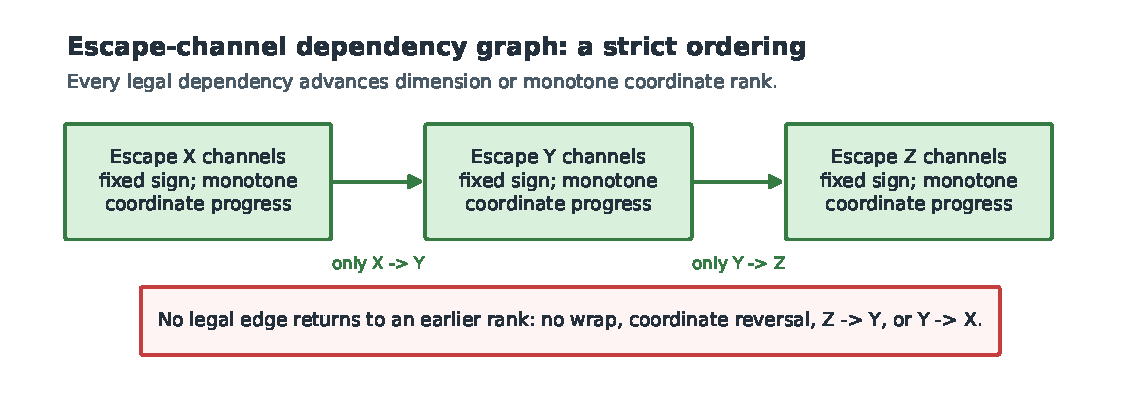
\includegraphics[width=\linewidth]{escape_cdg.pdf}
    \end{column}
    \begin{column}{0.34\textwidth}
      \begin{itemize}
        \item No wrap link or direction reversal.
        \item Dimension order: X, Y, then Z.
        \item Escape CDG is acyclic.
        \item Escape cannot return to adaptive channels.
      \end{itemize}
      \begin{block}{Result}
        A finite cyclic wait cannot remain after entering the Escape subnetwork.
      \end{block}
    \end{column}
  \end{columns}
\end{frame}

\begin{frame}{Topic 2: Critical Bubble Scheme (CBS)}
  \begin{columns}[T]
    \begin{column}{0.64\textwidth}
      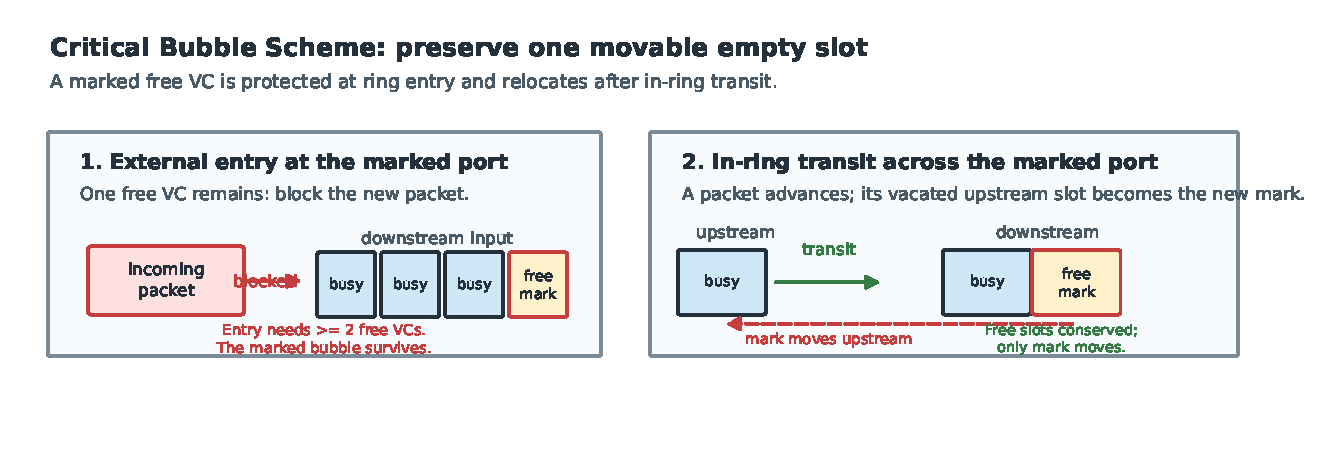
\includegraphics[width=\linewidth]{cbs_bubble.pdf}
    \end{column}
    \begin{column}{0.32\textwidth}
      \begin{itemize}
        \item DOR only, gated by \texttt{--enable-cbs}.
        \item Preserve one marked free buffer slot per directed ring.
        \item Ring entry needs two free VCs.
        \item In-ring transit moves the mark upstream.
      \end{itemize}
    \end{column}
  \end{columns}
\end{frame}

\begin{frame}{Two Complementary Safety Mechanisms}
  \footnotesize
  \begin{tabular}{p{0.18\linewidth}p{0.23\linewidth}p{0.23\linewidth}p{0.25\linewidth}}
    \toprule
    Mechanism & Protected mode & Resource cost & Safety invariant \\
    \midrule
    Escape VC & Adaptive Torus routing & Reserve $E\geq1$ VC per vnet & Packets never return from Escape to adaptive VCs. \\
    \addlinespace
    CBS & Torus DOR control traffic & No reserved VC & A marked free slot remains on every directed ring. \\
    \bottomrule
  \end{tabular}
  \vspace{0.55cm}
  \begin{block}{Different proof objects}
    Escape VC eliminates a channel-dependency cycle. CBS prevents a directed ring from becoming completely full.
  \end{block}
\end{frame}

\begin{frame}{Evaluation Methodology}
  \begin{itemize}
    \item 64 routers, four VCs per vnet, single-flit vnet-0 control traffic.
    \item Main sweep: 10,000 Ruby cycles, four patterns: uniform random, neighbour, tornado, and transpose.
    \item Throughput is received packets/node/Ruby-cycle; source acceptance detects injection backpressure.
    \item Fixed-VC ablation: 4A/0E, 3A/1E, 2A/2E, 1A/3E.
    \item CBS sweep compares DOR baseline with DOR+CBS under the same settings.
  \end{itemize}
\end{frame}

\begin{frame}{Topic 1 Results: Adaptive Routing}
  \begin{columns}[T]
    \begin{column}{0.60\textwidth}
      
\includegraphics[width=\linewidth]{latency_throughput.pdf}
    \end{column}
    \begin{column}{0.36\textwidth}
      \begin{tabular}{lrr}
        \toprule
        Mode & Stable TP & Hops \\
        \midrule
        Mesh XYZ & 0.210 & 3.763 \\
        Torus DOR & 0.237 & 3.006 \\
        Adaptive & 0.499 & 3.006 \\
        \bottomrule
      \end{tabular}
      \vspace{0.35cm}
      \begin{itemize}
        \item Transpose traffic.
        \item Adaptive: 2.10x DOR throughput.
        \item Escape use stays low: 0.34\% of transpose hops at full load.
      \end{itemize}
    \end{column}
  \end{columns}
\end{frame}

\begin{frame}{Topic 2 Results: CBS Flow Control}
  \begin{columns}[T]
    \begin{column}{0.60\textwidth}
      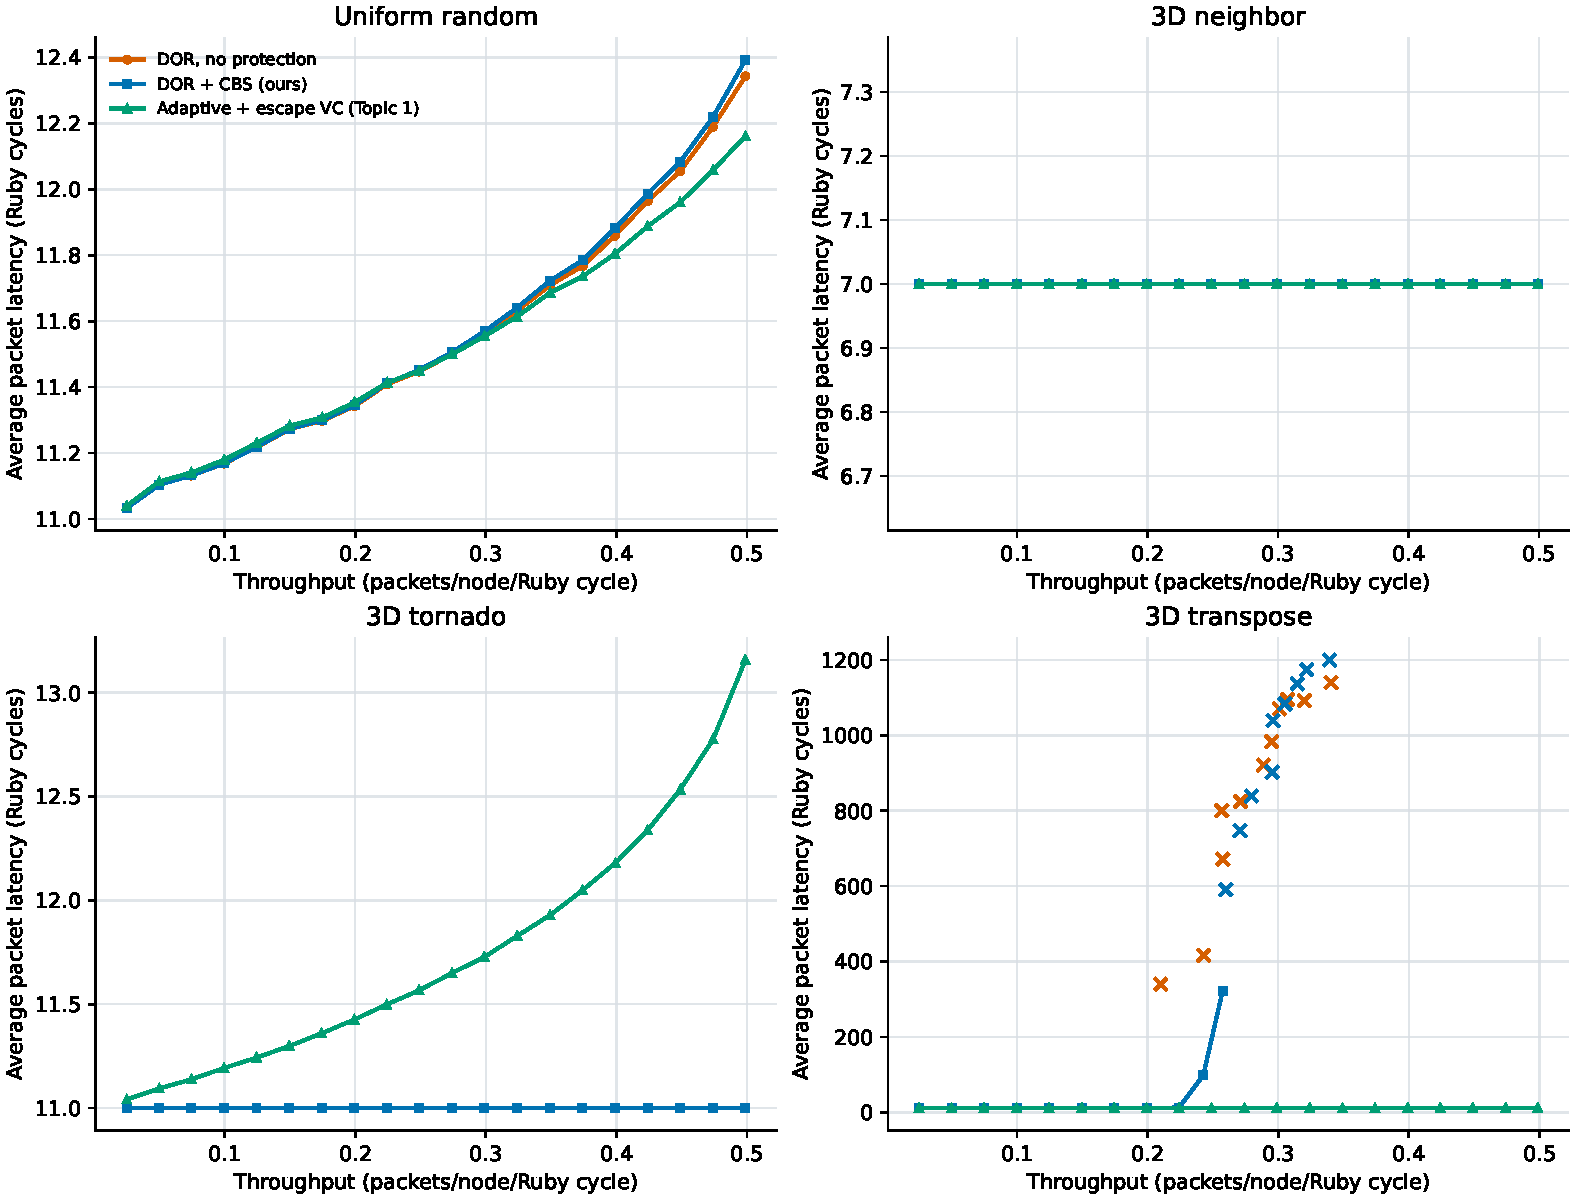
\includegraphics[width=\linewidth]{latency_throughput_topic2.pdf}
    \end{column}
    \begin{column}{0.36\textwidth}
      \begin{itemize}
        \item CBS keeps all four VCs available to DOR.
        \item On transpose, maximum stable throughput rises from 0.224 to 0.258 packets/node/Ruby-cycle.
        \item This is a 14.9\% improvement.
        \item On other patterns, full-load latency changes by at most 0.049 cycles.
      \end{itemize}
    \end{column}
  \end{columns}
\end{frame}

\begin{frame}{Division of Labor and Deliverables}
  \centering
\includegraphics[height=0.24in]{member_names.pdf}
  \vspace{0.2cm}
  \begin{columns}[T]
    \begin{column}{0.47\textwidth}
      \textbf{Changxun Pan}
      \begin{itemize}
        \item 3D Mesh/Torus topology and routing modes.
        \item Adaptive and Escape-VC design, experiments, and progress argument.
        \item Topic 1 figures and report sections.
      \end{itemize}
    \end{column}
    \begin{column}{0.47\textwidth}
      \textbf{Liming Wang}
      \begin{itemize}
        \item CBS state, allocator rules, and statistics.
        \item Topic 2 experiments, figures, and correctness argument.
        \item Report integration and validation.
      \end{itemize}
    \end{column}
  \end{columns}
  \vspace{0.2cm}
  \begin{block}{Shared}
    Evaluation methodology, code review, final report, and presentation.
  \end{block}
\end{frame}

\begin{frame}{Conclusion}
  \begin{itemize}
    \item A 3D Torus implementation exposes useful path diversity but needs explicit deadlock control.
    \item Escape VCs provide a low-use, acyclic progress path for minimal adaptive routing.
    \item CBS provides an alternative for DOR: no reserved VC, but a conserved critical bubble per directed ring.
    \item Both mechanisms are implemented, measured, and accompanied by an invariant-based safety argument.
  \end{itemize}
  \vfill
  \centering\Large Questions
\end{frame}

\end{document}
